\subsection{Incremental value beyond the profitable commercial core}

The positive Beta commercial result does not depend on the following enhancements. The same 768 confirmation histories separately test whether the shared graph increases enterprise surplus. No primary scenario establishes that additional benefit. Declining retention or continuing with existing frontier capabilities preserves the profitable operating option; it is not a failed enterprise. All values remain conditional model results, not realized margins or empirical demand estimates.

\begin{table}[H]\centering\small\caption{Same-policy enterprise comparison, USD. The interval is for the paired network-minus-Beta increment.}\label{tab:primary}

\begin{tabular}{lrrrr}\toprule Scenario & Beta & Network & Increment & 95\% MC interval\\\midrule

Conservative & 411,421 & 397,474 & -13,947 & [-14,104, -13,790] \\

Central & 3,702,395 & 3,690,332 & -12,063 & [-18,516, -5,610] \\

Favorable & 6,763,479 & 6,754,714 & -8,766 & [-118,842, 101,310] \\

\bottomrule\end{tabular}\end{table}

The conservative policy uses the adaptive price rule with zero offset and chooses delivery only; its mean offer is 29.8\% of the scope-matched human reference. Central selection chooses a fixed 55\% price and delivery only. Favorable selection chooses a fixed 75\% price, retention hurdle 1.5, and no separate R\&D. These discounts emerge from the finite search. They were not imposed. Fixed-price selection does not establish that a fixed price is universally best.

No primary history makes a separate C investment. Network and network-without-C results are therefore identical. Conservative and central policies do not retain graph capabilities; operating the available network still incurs overhead and can shift cash timing. Their small outcome differences cannot be called Alpha. A manager could avoid that unused service by operating the Beta-only configuration; the experiment deliberately reports its cost.

\begin{figure}[H]\centering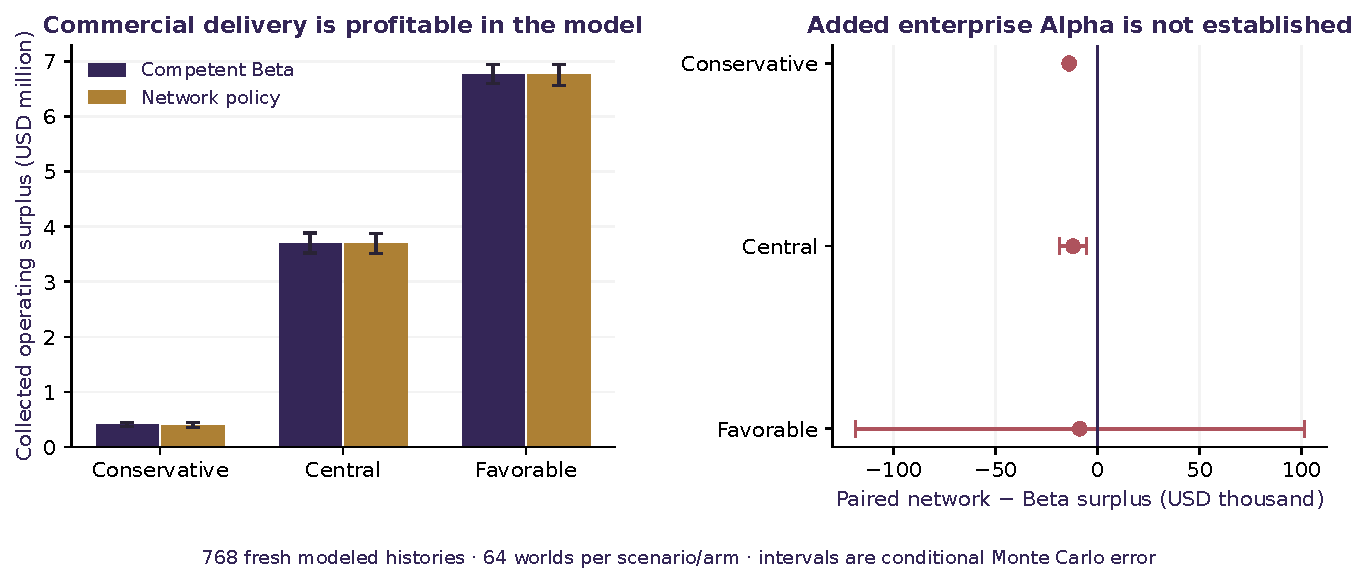
\includegraphics[width=\linewidth]{figures/economics.pdf}\caption{Primary modeled commercial results and their internal increment. Large absolute surplus does not establish a shared-capability advantage.}\end{figure}

In the favorable condition, the network averages 7.84 retention campaigns, 7.38 admissions and 44.84 useful recipient jobs per world. Those are adoption and activity counts, not added outcomes. Its accepted-useful outcome difference from Beta is $-0.875$ jobs (95\% conditional MC interval $[-4.034,2.284]$). The surplus difference is unresolved and has a negative point estimate. The network-minus-isolated comparison is also unresolved: USD$-51,118$ with interval $[-180,073,77,838]$. Selection on training data does not guarantee a confirmation gain.

\subsection{Complete costs, cash and the source of retained learning}

\begin{table}[H]\centering\small\caption{Mean network cost books and collections, USD. Common costs are charged once; B includes graph overhead even without retained skills.}

\begin{tabular}{lrrrrr}\toprule Scenario & Collections & A jobs & B retention & C new R\&D & Common\\\midrule

Conservative & 677,726 & 209,639 & 13,870 & 0 & 56,744 \\

Central & 4,194,516 & 431,819 & 14,197 & 0 & 57,696 \\

Favorable & 7,368,084 & 523,584 & 31,711 & 0 & 58,076 \\

\bottomrule\end{tabular}\end{table}

Closing obligations average USD471 in central network runs and zero in the other two; they are deducted in surplus. Seed capital is additional cash, not revenue. All 64 network worlds in each scenario have positive surplus and no recorded cash shortfall. Zero shortfalls in 64 worlds still has a 95\% Wilson upper bound of 5.66\%; it is not proof of a sub-5\% real-world risk.

The independent retained-ledger audit reconciles every one of the 768 confirmation worlds, including expense-book partition, commitments, warranties, collection delays, source-job memos and finite cash. It found no invariant failure. These repeated accounting checks verify the implementation, not the truth of the workload or demand assumptions.

Across favorable network worlds, 502 B campaigns occur. Of these, 396 are labeled funded from available operating surplus and 106 from seed or mixed funds. Source-job collection often comes after retention: 381 recorded source links collect later, 132 before or at retention, and 9 remain uncollected at closing. A customer order therefore does not imply that its receipt financed the next extraction.

An illustrative trace uses the prespecified first favorable network world, seed 770001. Source job 9 incurs USD974.32 of direct A cost, including a USD536.53 learning memo that is already inside that cost. Retention reserves USD183.94 at week 5 and spends it at week 6: USD58.94 extraction and USD125 creator bounty. A separate USD51.30 portfolio appraisal occurs in week 5; ongoing maintenance and network service also remain in B. The reserved campaign subtotal is not its full lifecycle cost. Its USD18,996.75 customer collection arrives at week 7. The first useful receiving job in this lineage completes at week 13. This early retention is seed/mixed-funded. No source A amount is charged again. The sequence illustrates the modeled lifecycle; it does not prove that this receiver could not have succeeded with competent reconstruction, and this entire network world earns USD1,062,359 less than its paired Beta world.

Validation remains imperfect. Conservative, central and favorable network worlds average 5.23, 7.00 and 5.70 false passes respectively. Remediation costs are charged, but these errors and the finite liability assumptions prevent treating modeled profitability as operational service qualification.

\subsection{A conditional recipient-level Alpha result}

The separate deterministic recipient panel holds the task and resources fixed. Its five competent recipient profiles yield expected initial delivery savings of USD750.08, USD148.43, zero, USD505.78 and zero. The specialist and already-equivalent recipient decline acquisition; missing a skill file does not imply missing capability. Every declared delivery route remains feasible in this panel, so it demonstrates no newly feasible job.

At the declared 80 uses, the paid-job-retention panel projects USD34,740.79 less complete delivery cost and USD9,495.70 additional lifecycle cost, leaving USD25,245.09 modeled net Alpha. Remaining upfront B is USD849.84; upkeep, revalidation and reassessment dominate the rest. Historical A is unspecified in this panel, retained as a memo, and never charged again. Its uncertainty allowance is zero; this arithmetic is not a measured or statistically confirmed return.

The illustrative optional new-R\&D campaign instead projects USD$-5,295.69$. It assumes one failed construction attempt (USD11,617.10 within USD23,234.20 total C construction) and campaign success 0.648, versus 0.90 for retention. This is not a cost-only matched contrast or evidence that new R\&D generally fails. The strict reuse thresholds at the declared lifetime are 22 uses for retention and 97 for new R\&D. These thresholds keep the declared age/task mixture; they are not interchangeable with the enterprise's component-level screening. A first positive projected lifetime of two weeks in the retention panel is a prospective utility threshold, not an observed two-week cash repayment.

\begin{figure}[H]\centering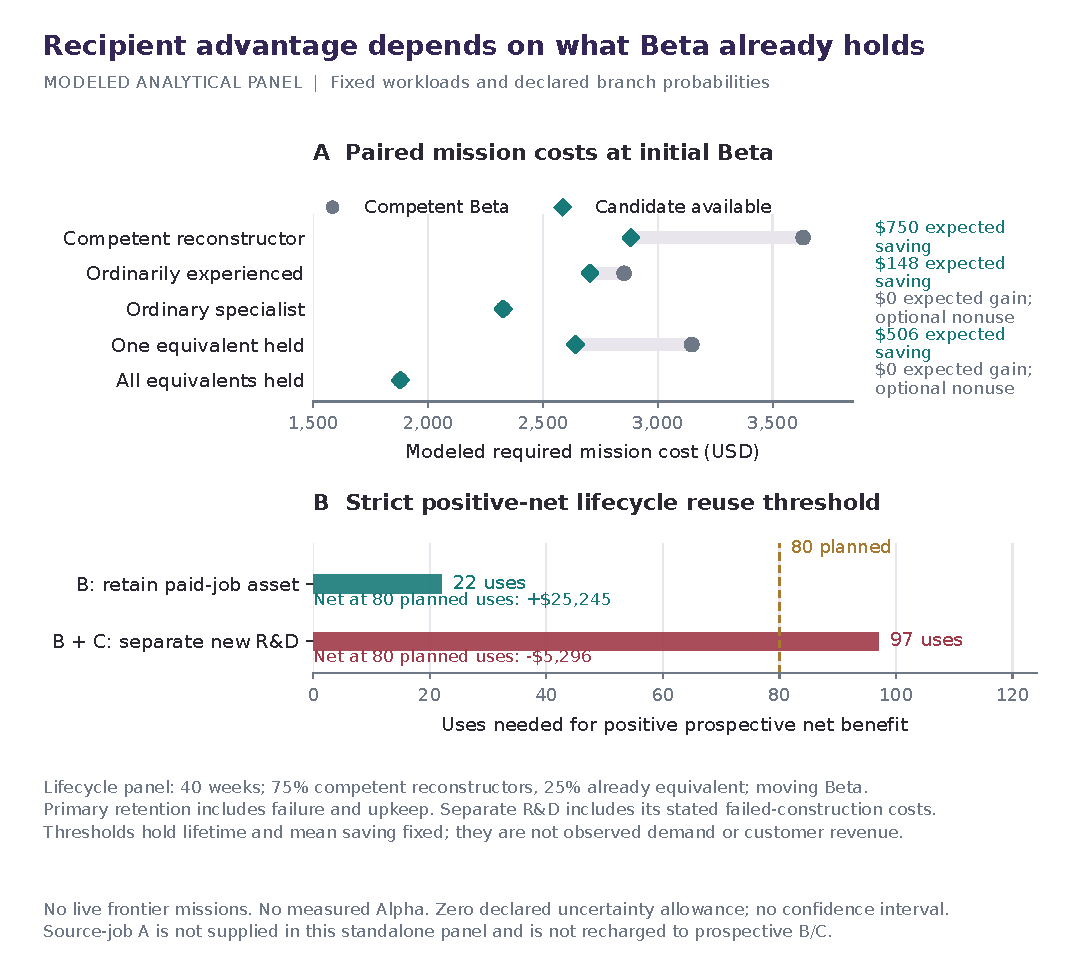
\includegraphics[width=\linewidth]{figures/recipients.pdf}\caption{Separate deterministic modeled recipient probes. Existing equivalents and optional nonuse are preserved. These values do not repair the unresolved enterprise comparison.}\end{figure}

The actual graph adapter admits the positive modeled bundle and rejects optional new R\&D into separate failure memory, using distinct fixture producer, validators and admitter. Six authenticated direct-label fixture members retrieve it; lacking an action permission blocks an execution permit while preserving access. A declared Beta change invalidates its old authority. This establishes a source-bound software lifecycle over modeled evidence, not operational Alpha.

\subsection{Sensitivity, demand and capacity}

All 2,736 predeclared sensitivity histories and 240 ablation histories completed. Sensitivities explicitly enable optional B retention under the frozen central pricing rule; they are not the central delivery-only policy relabeled as a success. Separate-C-enabled responses are retained alongside no-C responses. Their finite grids describe conditional mechanisms and parameter sensitivity, not market confidence or a universal optimum. Intervals are pointwise normal Monte Carlo intervals without multiplicity correction.

\begin{figure}[H]\centering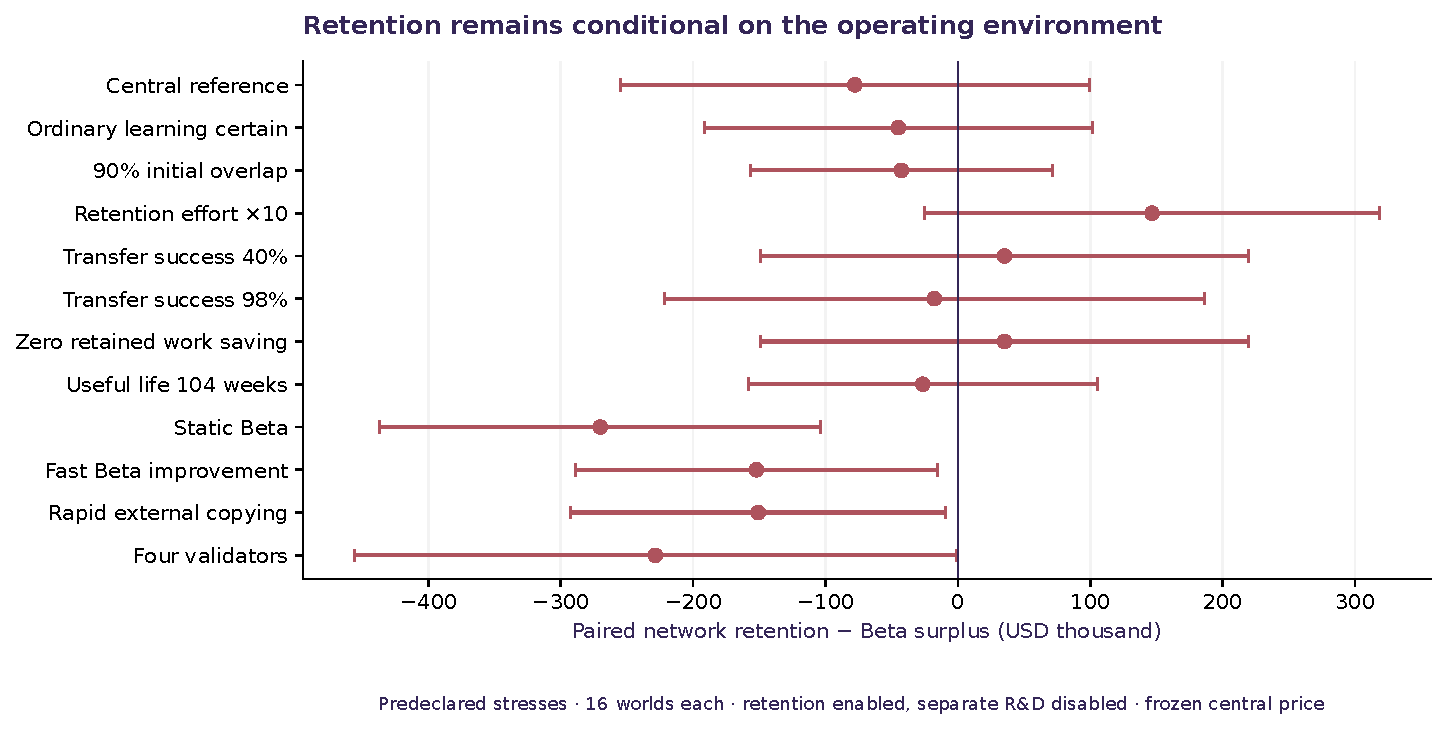
\includegraphics[width=\linewidth]{figures/sensitivity.pdf}\caption{Selected predeclared stresses. Bars are paired conditional Monte Carlo intervals across 16 independent modeled worlds; all 57 cases remain in the companion.}\end{figure}

\begin{table}[H]\centering\small\caption{Selected conditional stresses, USD mean surplus and paired increment.}

\begin{tabular}{lrrr}\toprule Stress & Network & Network $-$ Beta & 95\% MC interval\\\midrule

Central, B enabled & 3,322,575 & -77,839 & [-255,085, 99,406] \\

Human reference at 10\% & 55,483 & -24,721 & [-38,251, -11,191] \\

B effort $10\times$ & 3,547,114 & 146,700 & [-25,016, 318,415] \\

90\% overlap & 3,655,114 & -42,716 & [-156,919, 71,488] \\

Faster Beta & 3,496,427 & -152,226 & [-288,873, -15,579] \\

104-week useful life & 3,373,915 & -26,499 & [-158,373, 105,375] \\

Joint commercial downside & -18,757 & -2,096 & [-2,096, -2,096] \\

\bottomrule\end{tabular}\end{table}

\begin{figure}[H]\centering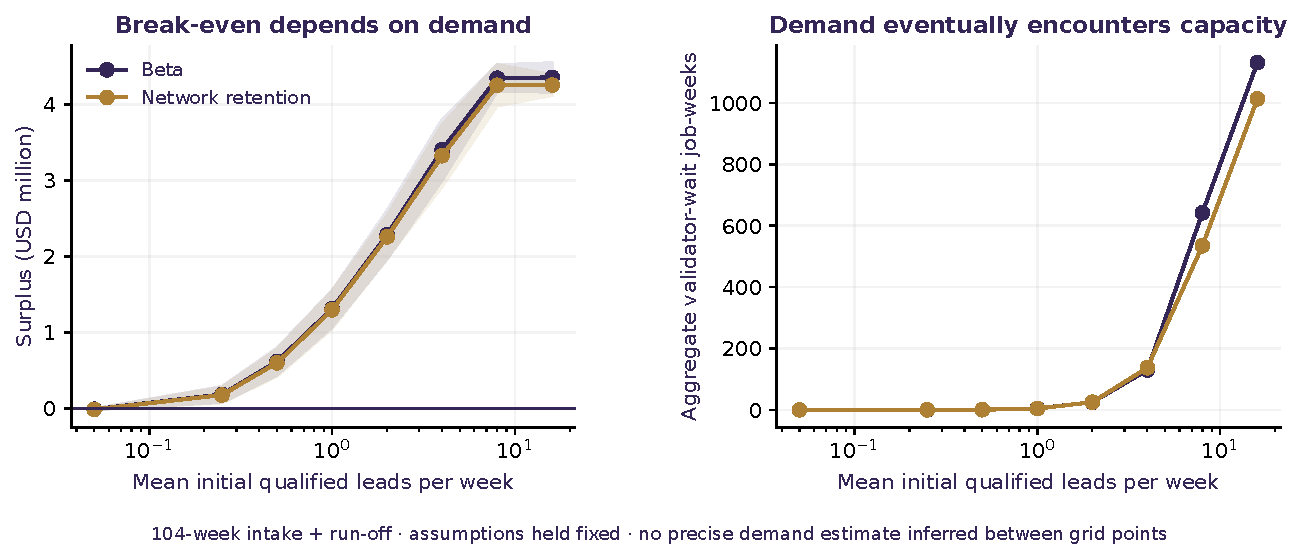
\includegraphics[width=\linewidth]{figures/demand.pdf}\caption{Demand and queueing under unchanged prices and other scenario assumptions. Aggregate waiting sums time across jobs; it can exceed the calendar horizon.}\end{figure}

For beta under the demand sweep, the modeled mean-profit sign changes between 0.05 and 0.25 initial qualified leads per week. No precise break-even arrival rate is identified between these grid points.

For network under the demand sweep, the modeled mean-profit sign changes between 0.05 and 0.25 initial qualified leads per week. No precise break-even arrival rate is identified between these grid points.

The split-sample initial-capacity menu selects scale complete double for beta. Its eight fresh test worlds give mean gain USD1,331,416 relative to the central capacity, with conditional interval [685,519, 1,977,314]. This tests the chosen starting configuration, not globally optimal expansion timing.

The split-sample initial-capacity menu selects scale complete double for network. Its eight fresh test worlds give mean gain USD1,448,477 relative to the central capacity, with conditional interval [890,348, 2,006,607]. This tests the chosen starting configuration, not globally optimal expansion timing.

\subsection{Counterfactuals and the moving frontier}

The component-removal and duplicate controls use the same initial resources and seeds. Central and conservative policies retain no graph capabilities, so component-removal effects there cannot establish a skill mechanism. The deliberately forgetful no-retention diagnostic is not the fair Beta comparator; ordinary competent learning remains in all primary comparisons.

\begin{table}[H]\centering\small\caption{Favorable component controls: network minus altered network, first 16 confirmation seeds.}

\begin{tabular}{lrr}\toprule Control & Mean surplus difference (USD) & 95\% MC interval\\\midrule

remove representation & 1,591,250 & [1,215,509, 1,966,990] \\

remove falsifier & 607,215 & [354,033, 860,397] \\

remove composition & 13,805 & [-17,871, 45,480] \\

duplicate & 94,431 & [-84,834, 273,697] \\

no retention & 407,496 & [155,367, 659,625] \\

\bottomrule\end{tabular}\end{table}

\begin{figure}[H]\centering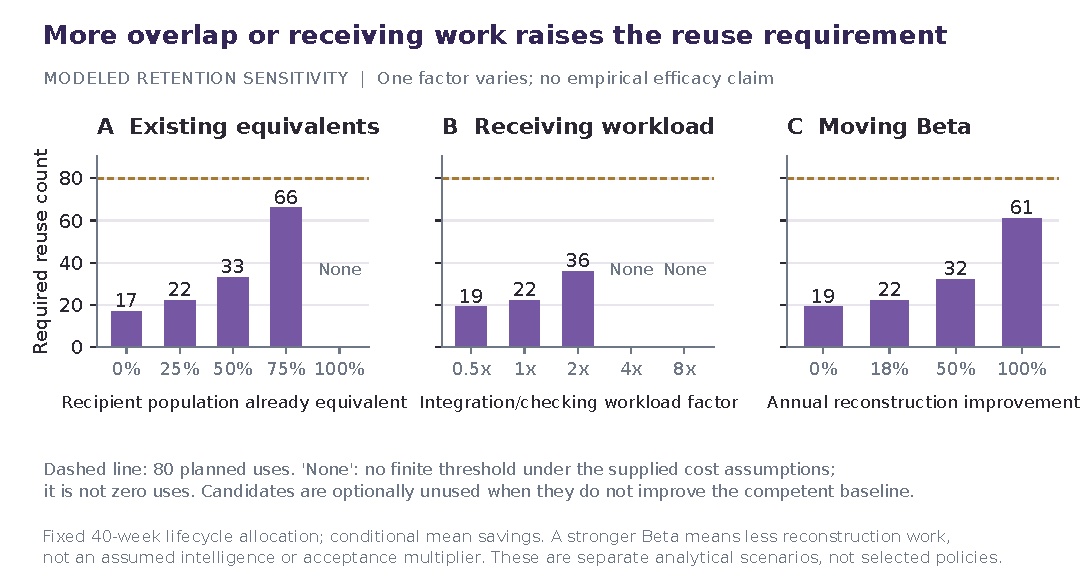
\includegraphics[width=.95\linewidth]{figures/recipient_thresholds.pdf}\caption{The separate recipient panel exposes how overlap, checking and improved Beta raise the strict reuse threshold. No finite threshold remains a distinct negative result.}\end{figure}

Large representation and falsifier removal losses are total intervention effects. The removal masks runtime eligibility while prospective appraisal can still value the removed component, allowing futile retention attempts and changed routing or queues. These controls diagnose dependence and policy brittleness; they are not clean estimates of a component's isolated net Alpha and do not overturn the fair Beta comparison. The duplicate control explicitly marks the proposed asset redundant, testing rejection mechanics rather than independently discovering the frequency of redundancy.

Among the 57 retention-versus-Beta stresses, the only positive paired interval occurs at USD10,000 seed. Both arms suffer cash shortfall in all 16 worlds and retain no capability; the USD334 difference is a smaller failure loss, not Alpha. Fast Beta and rapid copying instead produce negative retention increments. Some optional-C enablement contrasts are positive despite zero C campaigns in those conditions: evaluator overhead and timing can change outcomes without producing a new asset. The complete corpus records three C campaign events in reduced-construction-cost conditions, not three independent invention replications: one seed appears in two alternative conditions. It establishes no separate-R\&D capability feedback loop.

The commercial core is a positive modeled finding within its stated assumptions. The optional capability result is narrower: paid-job accounting can make remaining retention much less expensive than a new invention campaign, and the executable system can test and enforce a conditional Alpha claim. Full overhead, capacity, adaptation and demand still determine whether that enhancement pays. This edition does not establish a durable moat, a new commercially validated offering unlocked by sharing, an extra-R\&D feedback loop or self-acceleration. None is required for profitable Beta delivery.
